\chapter{Introduzione}

\section{Il problema}

In ambito universitario è problematica molto comune quella di cercare di assegnare aule a 
gruppi di studenti in modo tale da rispettare le richieste in numero di posti
di ciascuno di essi senza nemmeno concretamente conoscere il numero di allievi che frequenteranno 
realmente il corso in questione, dovendo l'istituto assegnarle in anticipo rispetto all'inizio
delle lezioni.

Si pone quindi l'ulteriore problema di facilitare la raccolta di dati che permetta di effettuare 
delle stime più accurate, quindi di registrare in modo automatico la partecipazione degli universitari
a ciascuna lezione e quindi inferire attraverso di essi queste stime.

\medskip

Quest'applicazione si pone l'obiettivo di risolvere esattamente questa problematica (il funzionamento è 
illustrato in \ref{fig:app_flow}):
a partire da foto (che si intende essere di aule) riconosce il numero di volti e quindi di studenti in essa 
presenti. Questa informazione, associata ad informazioni riguardanti la lezione in questione, viene fornita 
insieme a quest'ultime ad uno stimatore che, in base ai dati ricevuti cerca di costruire un modello matematico 
capace di stimare il flusso di allievi in nuove e richieste situazioni: delle stime che verranno impiegate 
per distribuire ciascun gruppo nelle diverse aule con data capacità in modo ottimale, cercando cioè di 
massimizzare il valore di una certa funzione matematica che rappresenta il problema di allocazione. 

\begin{figure}
    \begin{small}
        \begin{center}
            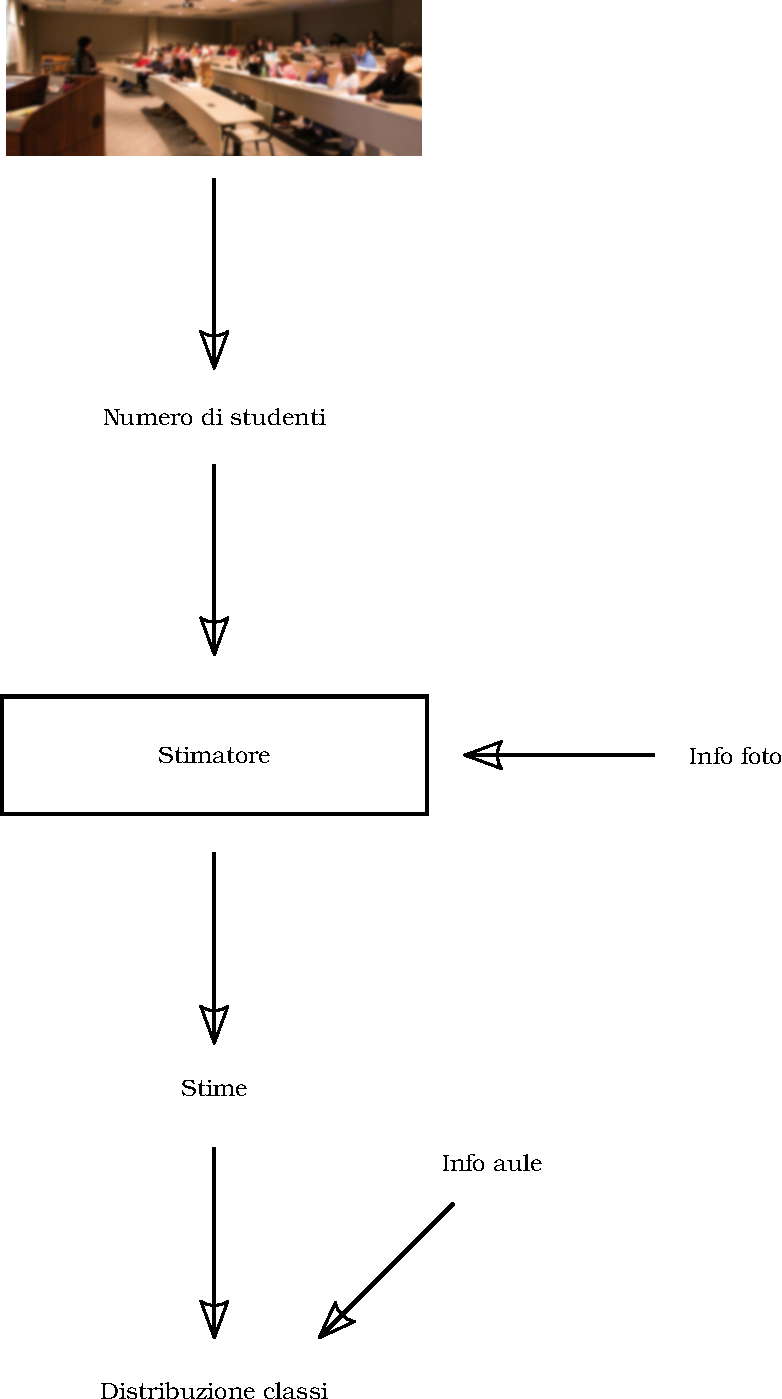
\includegraphics[width=0.70\textwidth]{app_flow.pdf}
        \end{center}
        \caption{Il flusso di funzionamento dell'applicazione}
        \label{fig:app_flow}
    \end{small}
\end{figure}

\section{Struttura del documento}

Il documento è strutturato in 

\begin{itemize}
    \item \textbf{State of the Art}, in cui vengono accennati i concetti teorici utilizzati per la risoluzione 
        del problema; vengono analizzati articoli e fonti che hanno affrontato le stesse problematiche. 
    \item \textbf{Metodo}, nel quale sono approfondite le metodologie usate per la realizzazione 
        dell'applicazione e vengono trattate ulteriori questioni sorte nell'implementazione.
    \item \textbf{Risultati}, che illustra gli esiti e l'efficienza della realizzazione scelta.
    \item \textbf{Conclusioni}, contenente le osservazioni finali dedotte dai risultati ottenuti.
\end{itemize}

\section{Codice sorgente}

Il codice completo di questa applicazione è accessibile su GitHub al seguente 
indirizzo 

\begin{center}
    \url{https://github.com/morpheusthewhite/celephais/}; 
\end{center}

\noindent
analogamente è stato pubblicato il codice \LaTeX di questa tesi al link 

\begin{center}
    \url{https://github.com/morpheusthewhite/bachelor-thesis}.     
\end{center}
